\section{Proposed Method}
\label{sec:method}

\subsection{Architecture Overview}
The system architecture of the proposed \method\ framework is illustrated in Fig.~\ref{fig:overview}. The framework comprises three operational stages: 
\begin{enumerate}
    \item \textbf{Offline Privileged Training}: A global teacher policy $\pi_T$ is trained via reinforcement learning utilizing privileged global graph topology information.
    \item \textbf{Global-to-Local Knowledge Distillation}: The trained teacher is frozen, and its soft next-hop selection probabilities are distilled into a local student policy $\pi_S$, which operates solely on 1-hop candidate features.
    \item \textbf{Predictive Risk Switching (PRS) Execution}: During online deployment on UAVs, the final routing action is selected by a risk switch that dynamically toggles between the nominal distilled student policy and a predictive safety branch based on real-time link and queue danger indicators.
\end{enumerate}

\begin{figure*}[t]
\centering
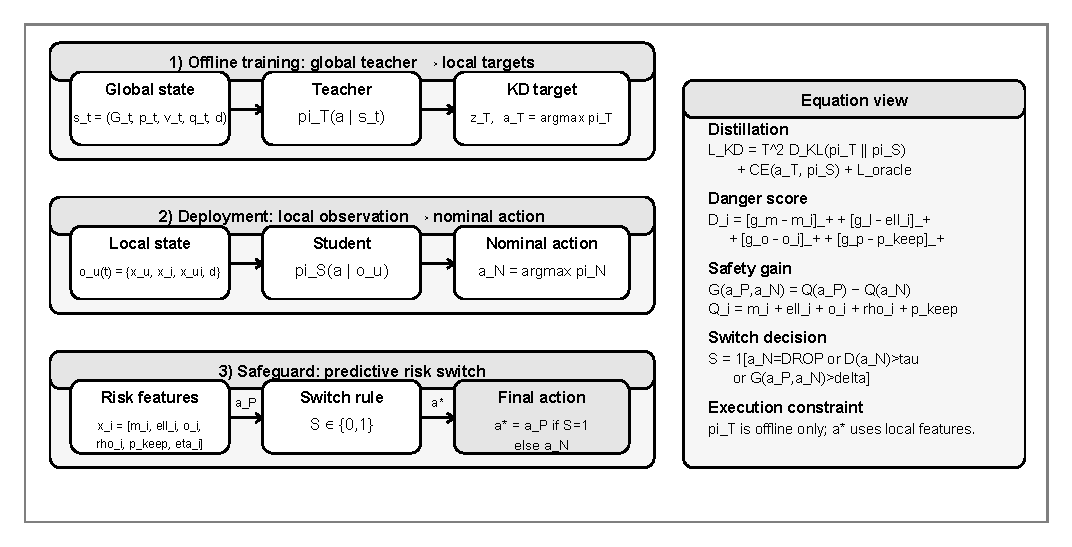
\includegraphics[width=0.96\textwidth]{figures/method_overview_pub.pdf}
\caption{System architecture of the proposed GLOBE++ Lite-P+ routing pipeline. The global teacher is used only for offline privileged training and distillation, while the deployed router selects the next hop from local one-hop observations through a nominal branch, a predictive branch, and a risk-switch decision.}
\label{fig:overview}
\end{figure*}

\subsection{Reinforcement-Learning-Based Global Teacher Training}
The global teacher policy $\pi_T(a \mid s_t; \theta_T)$ parameterizes the probability distribution over the forwarding candidates using parameters $\theta_T$. During offline training, the teacher observes the full global network state:
\begin{equation}
    s_t = (\mathcal{G}_t, p_t, v_t, q_t, d) \in \mathcal{S},
\end{equation}
enabling the actor-critic network to gain global awareness of routing paths and congestion profiles across the entire network. At each routing hop, the teacher samples a forwarding node:
\begin{equation}
    a_t \sim \pi_T(a_t \mid s_t; \theta_T).
\end{equation}

The teacher is optimized to maximize the expected discounted return:
\begin{equation}
    J(\theta_T) = \mathbb{E}_{\pi_T} \left[ \sum_{t=0}^{T_{\mathrm{ep}}} \gamma^t r_t \right],
\end{equation}
where the single-hop routing reward $r_t$ is defined as:
\begin{equation}
    r_t = \alpha_{\mathrm{succ}}R_{\mathrm{succ}} - \alpha_D D_t - \alpha_E E_t - \alpha_H H_t - \alpha_F F_t.
\end{equation}
Here, $R_{\mathrm{succ}} \in \{0, 1\}$ indicates packet arrival, $D_t$ represents single-hop propagation and queuing delay, $E_t$ is the estimated transmission power consumption, $H_t = 1$ penalizes unnecessary hops, and $F_t$ represents failure penalties for packet drops or routing loop occurrences.

The policy parameters $\theta_T$ are optimized using Proximal Policy Optimization (PPO). The probability ratio of the policy update is:
\begin{equation}
    \rho_t(\theta_T) = \frac{\pi_T(a_t \mid s_t; \theta_T)}{\pi_T(a_t \mid s_t; \theta_T^{\mathrm{old}})}.
\end{equation}
Let $A_t$ be the generalized advantage estimator:
\begin{equation}
    A_t = \hat{R}_t - V_T(s_t; \phi_T),
\end{equation}
where $\hat{R}_t$ is the empirical discounted return and $V_T(s_t; \phi_T)$ is the parameterized value function baseline. The clipped surrogate policy loss is:
\begin{equation}
    \mathcal{L}_{\mathrm{PPO}}(\theta_T) = - \mathbb{E}_t \left[ \min \left( \rho_t(\theta_T)A_t, \; \mathrm{clip}(\rho_t(\theta_T), 1-\epsilon, 1+\epsilon)A_t \right) \right],
\end{equation}
where the clipping coefficient $\epsilon \in (0, 1)$ stabilizes training updates. The value function parameter $\phi_T$ is trained via mean squared error:
\begin{equation}
    \mathcal{L}_{V}(\phi_T) = \mathbb{E}_t \left[ \left( V_T(s_t; \phi_T) - \hat{R}_t \right)^2 \right].
\end{equation}
Combining these, the complete loss function for training the global teacher is:
\begin{equation}
    \mathcal{L}_{T}(\theta_T, \phi_T) = \mathcal{L}_{\mathrm{PPO}}(\theta_T) + c_V \mathcal{L}_{V}(\phi_T) - c_H \mathcal{H}(\pi_T(\cdot \mid s_t; \theta_T)),
\end{equation}
where $\mathcal{H}$ represents the policy entropy bonus scaled by hyperparameter $c_H$ to promote exploration.

\subsection{Global-to-Local Policy Distillation}
Once the teacher parameters converge to $\theta_T^\star$, they are frozen. A lightweight student network $\pi_S(a \mid o_u; \theta_S)$, represented as a Multi-Layer Perceptron (MLP), is trained to mimic the teacher's decisions using only local observations $o_u$. 

To perform distillation, we pass the logits of both the teacher ($z_T$) and student ($z_S$) through a softmax function with a distillation temperature $T \ge 1$, yielding soft action targets:
\begin{equation}
    y_T(a) = \mathrm{softmax}\left(\frac{z_T(a)}{T}\right), \quad y_S(a) = \mathrm{softmax}\left(\frac{z_S(a)}{T}\right).
\end{equation}
The distillation objective combines KL-divergence over soft probabilities, cross-entropy over hard teacher targets, and an oracle-directed shortest-path loss:
\begin{equation}
    \mathcal{L}_{\mathrm{KD}}(\theta_S) = \lambda_{\mathrm{KL}} T^2 D_{\mathrm{KL}}(y_T \Vert y_S) + \lambda_{\mathrm{CE}} \mathrm{CE}(a_T, \pi_S) + \lambda_{\mathrm{O}} \mathcal{L}_{\mathrm{oracle}},
\end{equation}
where $a_T = \arg\max_{a} \pi_T(a \mid s_t; \theta_T^\star)$ is the hard action selected by the teacher, and $\mathcal{L}_{\mathrm{oracle}}$ penalizes deviations from geometrically valid shortest-path routes to bound execution errors in unseen topologies.

\subsection{Predictive Candidate Features and P+ Extensions}
While the distilled student policy provides strong general routing behavior, it can fail near transient routing holes or during rapid link degradations. The proposed Phase 13 \method\ extension incorporates local predictive features to assess connection risks. For each candidate next-hop node $i \in \mathcal{N}_u(t)$, the nominal safety branch extracts basic risk features:
\begin{equation}
    x_i^{\mathrm{risk}} = [m_i, \ell_i, q_i, o_i],
\end{equation}
where $m_i$ is the RSSI link margin, $\ell_i$ is the predicted link lifetime, $q_i$ is the neighbor queue headroom, and $o_i$ is the onward link stability (best estimated link lifetime of node $i$'s outgoing links).

The P+ extension enriches this representation with four local metrics:
\begin{equation}
    x_i^{+} = [\bar{o}_{i,\mathrm{top}k}, \rho_i, p_{i,\mathrm{keep}}, \eta_i],
\end{equation}
where:
\begin{itemize}
    \item $\bar{o}_{i,\mathrm{top}k}$ is the average lifetime of node $i$'s top-$k$ onward links, preventing reliance on a single high-lifetime but high-variance link.
    \item $\rho_i$ is the normalized onward redundancy, reflecting the density of alternative next-hops available at node $i$.
    \item $p_{i,\mathrm{keep}}$ is the link survival probability, computed using a stochastic channel model to account for sudden blockages.
    \item $\eta_i = 1 - (d_i / R_c)^2$ is an energy-efficiency proxy based on the distance $d_i$ between node $u$ and node $i$.
\end{itemize}

\subsection{Danger Score and Safety Utility}
Using the P+ features, we define the candidate Danger Score $D_i$ for node $i$ as:
\begin{equation}
    D_i = [g_m - m_i]_+ + [g_\ell - \ell_i]_+ + [g_o - o_i]_+ + [g_k - \bar{o}_{i,\mathrm{top}k}]_+ + 0.5[g_\rho - \rho_i]_+ + [g_p - p_{i,\mathrm{keep}}]_+,
\end{equation}
where $[x]_+ = \max(x, 0)$ and the $g$ parameters ($g_m, g_\ell, g_o, g_k, g_\rho, g_p$) represent predefined safety thresholds (gates) for each feature. Correspondingly, the Safety Utility $Q_i$ is defined as the sum of link quality metrics:
\begin{equation}
    Q_i = m_i + \ell_i + o_i + \bar{o}_{i,\mathrm{top}k} + 0.5\rho_i + p_{i,\mathrm{keep}}.
\end{equation}

For a nominal candidate action $a_N \sim \pi_S$ and a predictive candidate action $a_P$ proposed by the risk branch, the Safety Gain is:
\begin{equation}
    G(a_P, a_N) = Q_{a_P} - Q_{a_N}.
\end{equation}

\subsection{Risk-Switch Decision Logic}
The PRS module utilizes the nominal action $a_N$ by default. The predictive branch $a_P$ is activated to select an alternative next-hop only when the nominal action is diagnosed as unsafe. The PRS activation indicator $S \in \{0, 1\}$ is computed as:
\begin{equation}
    S = \mathbb{1}\left[ a_N = \dropact \quad \lor \quad D_{a_N} > \tau \quad \lor \quad \left( a_P \neq a_N \; \land \; G(a_P, a_N) > \delta \; \land \; D_{a_P} < D_{a_N} \right) \right],
\end{equation}
where $\tau$ is the maximum tolerable danger threshold, and $\delta$ is the minimum required safety gain. The final routing action $a^\star$ is then formulated as:
\begin{equation}
    a^\star = \begin{cases} a_P, & S = 1, \\ a_N, & S = 0. \end{cases}
\end{equation}

\subsection{Energy-Aware Tie Breaking and Drop Suppression}
To optimize physical routing overhead, we introduce two logit adjustments in the student decision branch:
\begin{enumerate}
    \item \textbf{Energy-Aware Tie Breaking}: The predictive logit $z_i^P$ for candidate $i$ is adjusted using the energy proxy:
    \begin{equation}
        z_i^{P+} = z_i^P + \lambda_E \eta_i,
    \end{equation}
    where $\lambda_E > 0$ forces the model to select geographically shorter and energy-efficient links when safety profiles are statistically similar.
    \item \textbf{Drop Suppression}: When at least one neighbor node passes the basic safety gate, the logit of the drop action is penalized:
    \begin{equation}
        z_{\dropact}^{P+} = z_{\dropact} - \lambda_D,
    \end{equation}
    where $\lambda_D > 0$ prevents premature packet discarding when viable, safe routes are locally available.
\end{enumerate}

Detailed execution flow of \method\ is provided in Algorithm~\ref{alg:risk_switch}.

